% \documentclass[12pt, twoside]{article}
\usepackage[letterpaper, margin=1in, headsep=0.2in]{geometry}
\setlength{\headheight}{0.6in}
%\usepackage[english]{babel}
\usepackage[utf8]{inputenc}
\usepackage{microtype}
\usepackage{amsmath}
\usepackage{amssymb}
%\usepackage{amsfonts}
\usepackage[nomessages]{fp} %\FPeval{\var-name}{2*sin(pi/6)}
\usepackage{siunitx} %units in math. eg 20\milli\meter
\usepackage{yhmath} % for arcs, overparenth command
\usepackage{tikz} %graphics
\usetikzlibrary{quotes, angles, arrows, arrows.meta}
\usepackage{graphicx} %consider setting \graphicspath{{images/}}
\usepackage{parskip} %no paragraph indent
\usepackage{enumitem}
\usepackage{multicol}
\usepackage{venndiagram}

\usepackage{fancyhdr}
\pagestyle{fancy}
\fancyhf{}
\renewcommand{\headrulewidth}{0pt} % disable the underline of the header
\raggedbottom
\hfuzz=2mm %suppresses overfull box warnings

\usepackage{hyperref}

\fancyhead[LE]{\thepage}
\fancyhead[RO]{\thepage \\ Name: \hspace{4cm} \,\\}
\fancyhead[LO]{BECA / Dr. Huson / Geometry\\*  Unit 13: Quadrilaterals \\* 27 March 2023}

\begin{document}

\subsubsection*{11.1 Parallelograms }
\begin{enumerate}
\item Given parallelogram $SNOW$ with $S(2,1),N(7,1),O(10,5),W(5,5)$
\begin{enumerate}
  \item Sketch $SNOW$, labeling the vertices.\\
    \begin{tikzpicture}[scale=.635]
      \draw [help lines] (-2,-1) grid (12,7);
      \draw [thick, ->] (-2.2,0) -- (12.4,0) node [below right] {$x$};
      \draw [thick, ->] (0,-1.2)--(0,7.4) node [left] {$y$};
    \end{tikzpicture}
  \item Find the area of the parallelogram.\vspace{3cm}
  \item Find the length of each side of the parallelogram.\vspace{5cm}
  \item Find the slopes of the diagonals, $\overline{SO}$ and $\overline{NW}$.\vspace{3.5cm}
  \item Are the diagonals parallel, perpendicular, or neither? Justify your answer.
  \end{enumerate}

  
\end{enumerate}
\end{document}
  